\chapter{SDN中流量测量的研究现状}\label{chap:sketch}

本章首先介绍了若干种典型的用于流量测量的sketch,并分别讨论它们的优点和缺点,
随后讨论流量测量的分布式部署,
最后对本文所要提出的sketch和分布式部署方案设立目标。

\section{现有的sketch测量方法}\label{sec:observation}
本节中,我们首先介绍以下4种现有的sketch,分别是:
Count-Min\cite{cormode2004improved}、CountSketch \cite{charikar2004finding}、Filtered Space-Saving \cite{homem2010finding}和SketchVisor \cite{huang2017sketchvisor}。
然后我们对这4中sketch的优势和不足进行讨论。

\subsection{Count-Min\cite{cormode2004improved}}

\begin{figure}[ht]
	\centering
	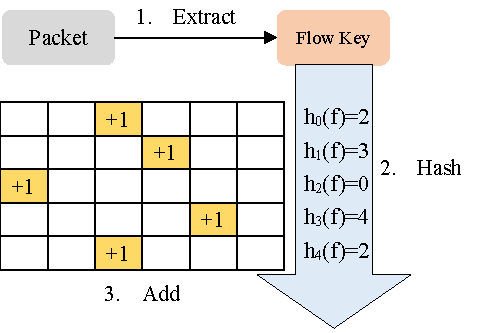
\includegraphics[width=0.7\linewidth]{fig/countmin2.pdf}
	\caption{Count-Min的更新过程}\label{fig:countmin}
\end{figure}

如图\ref{fig:countmin}所示,Count-Min sketch的存储形式是一个高度为$d$、长度为$w$的二维数组(这样的二维数组也称为\textit{bitmap})。数组中的每个位置称为一个“格子”(slot),格子中包含了一个从0开始的计数器。
数组中的每一行都拥有一个哈希函数,可以将任意流ID,如5元组,映射到$\{0,1,...,w-1\}$之间的某个整数。

当一个数据包到达时,Count-Min首先读取它的流ID,然后对于数组的每一行,使用它的哈希函数将ID映射为一个数,用这个数作为索引定位到相应的格子,将格子中的计数器增加对应的数据包大小。
由哈希函数的特性可知,同一条流的数据包将会一直映射到同样的$d$个格子。

要从Count-Min当中查询某个流的大小,先重复之前的步骤,利用哈希函数定位到具体的格子。因为Count-Min总共有$d$行,所以会找到$d$个格子。选择这些格子当中最小的计数器作为流的大小的估计。
由于哈希碰撞的存在,因此Count-Min的查询结果总是大于或等于实际的大小。

\subsection{CountSketch \cite{charikar2004finding}}\label{sec:countsketch}
CountSketch \cite{charikar2004finding}和Count-Min有一点相似,它同样拥有一个高度为$d$、长度为$w$的bitmap,以及$d$个将流ID映射成$\{0,1,...,w-1\}$中的整数的哈希函数。
除此之外,CountSketch还另有$d$个将流ID映射成$1$或$-1$的一系列哈希函数。

进行更新操作时,CountSketch首先使用第一套哈希函数来确定格子,再使用第二套哈希函数得到一个$1$或$-1$的系数。将数据包的大小乘上这个系数之后,再加到格子里的计数器上。
也就是说,Count-Min中的计数器只会增加,而CountSketch中的计数器有可能加也有可能减,取决于第二个哈希函数和流的ID。

在bitmap中查询流的大小的过程和Count-Min类似,但和Count-Min不同的是,CountSketch选择的不是$d$个计数值中的最小值,而是中位数。

\begin{figure}
   \centering
   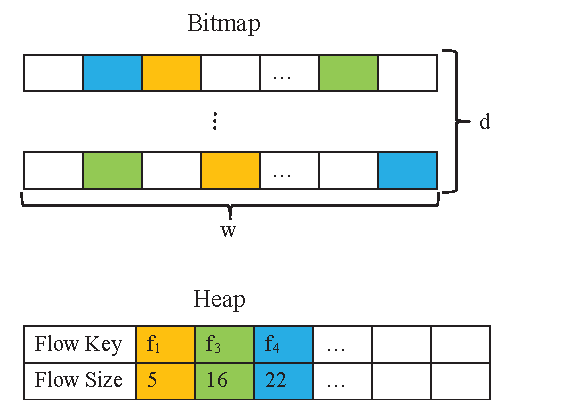
\includegraphics[width=0.7\linewidth]{fig/countsketch.pdf}
   \caption{CountSketch的结构}
   \label{fig:countsketch}
\end{figure}

此外,CountSketch还拥有找出top-$k$的流的能力。如图\ref{fig:countsketch}所示,为了记录top-$k$的流,CountSketch维护了一个容积为$k$的小根堆,其中存放了这些大流的ID以及它们的流量。

当数据包抵达时,CountSketch首先更新它的bitmap,然后再检查这个数据包所属的流是否已在堆中。
如果已在堆中,那么就将堆中对应的项目的流量值增加这个数据包的大小;
否则,CountSketch就会在bitmap中执行查询操作,获取当前流的流量估计值。
如果估计值比小根堆中最小的值要大的话,就将这个最小值移出堆,并将当前流的ID和流量估计值加入堆中。或者如果堆还没有满,也会当前流的信息放入堆中。

由于CountSketch的更新过程涉及堆的操作,因而它的计算负载也受堆操作的影响。如果使用简单的小根堆实现,那么更新堆中项目的时间复杂度是$O(\log{k})$, 在堆中查找某条流的时间复杂度是$O(k)$。
对每个数据包,CountSketch都要在堆中进行查找操作,这一过程大幅增大了CountSketch的计算负载。



\subsection{Filtered Space-Saving \cite{homem2010finding}}\label{sec:FSS}
在严格意义上,Filtered Space-Saving (FSS) \cite{homem2010finding}并非sketch,而应看做是一种基于“Counter”的算法,不过这个区别对于实际应用来说是可以忽略的。

FSS由一个只有1行的bitmap和一个容量为$k$的哈希表组成,其中bitmap用于粗略估算流的大小,哈希表则用来精确统计一部分的流的大小。
bitmap中的每个格子包括“计数器”和“指示器”两个字段。计数器用来记录流量统计,指示器则记录了通过哈希函数映射到这个格子中的流当中,有多少条也在哈希表当中。

每当新的数据包抵达,FSS首先用哈希函数将流的ID映射到bitmap中的一个格子,并检查这个格子中的指示器。
如果指示器的数字不为0,FSS会在哈希表中搜索该流ID。若流ID存在于哈希表中,那么哈希表中对应的计数器就增加数据包的大小。
如果指示器是0,或者ID不存在在哈希表中,那么就将bitmap中对应的格子里的计数器增加数据包的大小。
在此之后,若格子中的计数器大于哈希表中的最小值,就将该流的ID和计数器的数字插入哈希表中,并将格子中的指示器加1。
如果在插入时哈希表已满,那么哈希表中数值最小的一条流会被移除。在移除之后,FSS将会利用哈希函数为这条流找到它所对应的格子,将它原本在哈希表中的计数器数字复制到格子中的计数器中,并将格子里的指示器减1。

对于流ID存在于哈希表中的情况,FSS执行更新操作的时间复杂度是$O(1)$。其他情况下,FSS需要寻找哈希表中的最小项,因此时间复杂度是$O(k)$。

\begin{table}[h]
	\centering
	\begin{tabular}{c|c}
		\hline
		Kick-out 频率 & CPU周期/数据包 \\
		\hline
		0.1\% & 59 \\
		\hline
		0.5\% & 108 \\
		\hline
		1\% & 170 \\
		\hline
		2\% & 293 \\
		\hline
		5\% & 661 \\
		\hline
	\end{tabular}
	\caption{SketchVisor的计算负载随kick-out频率的变化}\label{tbl:sketchvisor}
\end{table}

\subsection{SketchVisor \cite{huang2017sketchvisor}}\label{subsec:sketchvisor}

SketchVisor \cite{huang2017sketchvisor}论文为其中的“Fast Path”设计了一个可以实现top-$k$流统计的算法。此算法维护一个有$k$行的表,表中的每一行包含一个流的ID和3个统计字段。
每到达一个数据包,如果该数据包的流存在于表中,或者表尚未存满,则只是简单的在表中插入或增加对应的表项。否则,整张表内的所有数据都要更新,这种操作被称为“kick-out”。
\cite{huang2017sketchvisor}中的测试结果显示,一个kick-out操作需要12332个CPU时钟周期,普通的更新则只需要47个时钟周期。

根据这一测试结果,我们估算了不同的kick-out比率下处理每个数据包消耗的平均时钟周期数。
如表\ref{tbl:sketchvisor}所示,SketchVisor的计算负载只在kick-out比率不超过1\%时才能够接受。也就是说,SketchVisor的表中所存储的流的流量之和要超过全部流量的99\%。
在实际网络中,由于流是在变化的,用一张表追踪99\%的流量明显不切实际。更何况要囊括更多的流,$k$也要随之增大,导致占用的内存空间也会增大。

\subsection{已有sketch所存在的问题}


在介绍了Count-Min等4种sketch之后,我们对这些sketch的优势和不足进行分析。

Count-Min的主要优势在于它的计算负载极低,并且估计误差较低。但是Count-Min并不记录任何流本身的信息,因而无法筛选出大流。一些研究对Count-Min进行了拓展,使其能够反查大流的信息。
如Deltoid \cite{cormode2005s}使用了额外的计数器来编码流的ID;
Reversible Sketch \cite{schweller2007reversible}将流ID拆分成多个部分并分别进行哈希;
FlowRadar \cite{li2016flowradar}使用连续的异或运算来编码和恢复流的ID。
然而,根据SketchVisor \cite{huang2017sketchvisor}中的测试结果,这些改进算法的计算负载都比较高。

SketchVisor有着较高的流量统计精度,然而它的计算负载取决于kick-out出现的频率。
随着kick-out比率的增加,SketchVisor的计算负载迅速增加并且变得无法负担。因而SketchVisor无法胜任大多数的应用情景。

CountSketch和FSS都使用了辅助数据结构,最坏情形下的更新操作的时间复杂度是$O(k)$。
第\ref{sec:simulation}节当中提供了一种用空间换时间的实现,使得最坏情形的时间复杂度降为$O(\log{k})$。
这个结果看起来似乎是可接受的,然而第\ref{sec:simulation}节中的模拟结果显示,这两种$O(\log{k})$的sketch的计算负载对于承载大量数据的交换机而言还是太大了。

我们用一个例子来帮助理解交换机的CPU资源与sketch的计算负载之间的关系。
假设一个交换机拥有24个端口,每个端口的速度都是10Gbps。所有端口的平均负载率记为$\beta$,这里假设$\beta$是0.2。数据包的平均大小是1KB。
可得交换机每秒要处理的数据包数约是:
\begin{equation}%\notag
    N = (10\times 10^9\cdot 24 \cdot \beta)/(0.5\times 10^3 \times 8) = 1.2\times 10^7
\end{equation}

在这样的假设下,如果sketch要处理经过交换机的所有数据包,那么sketch的吞吐量至少要能达到每秒1200万个数据包。
第\ref{sec:proto}节中我们对CountSketch和FSS的速度进行了测试,结果显示CountSketch和FSS处理一个数据包所需的CPU时钟周期数分别是约170和110。
假设这个交换机的CPU主频是1.5GHz,有2个物理核心(在市面上的交换机当中已经属于高端配置,相当于Juniper QFX5100系列\cite{juniper2018qfx5100}),CountSketch和FSS分别占用了68\%和44\%的CPU时间。
事实上,交换机的CPU还要承担其他的一些工作,比如流表的操作。
而且交换机上可能还会运行一些其他的服务,网络负载可能会比例子中的更高,这些因素要求了sketch的计算负载必须更低。



\section{流量测量的分布式部署}

如第\ref{sec:measurement}节所述,现有的基于流表的统计方式中,每个交换机都会统计经过它的所有数据包。
这种方法的可行性源于流表在数据包处理中不可或缺的地位:所有数据包到达时都要匹配流表,在匹配到的同时顺便更新统计数据。
也就是说,即使交换机不再进行流量统计,流表匹配仍旧是必须进行的,因而基于流表的流量统计带来的计算负载实际上微乎其微。

和流表相比,sketch面临的性能瓶颈要严重的多。
在第\ref{sec:observation}节当中我们假设,一个交换机需要每秒用一个双核1.5GHz的CPU处理1200万,即12Mpps(Packet per Second)。
但是对于交换机而言,每秒12M个数据包只能算是极低的工作负载。
例如Juniper QFX5100系列交换机配备了和假设中相同的双核1.5GHz的CPU,
然而根据其规格手册,该系列中所有型号的吞吐率都超过了10亿pps\cite{juniper2018qfx5100},相当于上述假设的近100倍。
部分型号更是达到了14.4亿pps的吞吐量。
通过简单的计算便可得出,要想让sketch能够在这颗CPU上达到10亿pps的吞吐量,处理每个数据包不能花费超过3个时钟周期。
Sketch是部署在SRAM上的,以Intel Haswell处理器为例,在L1缓存的SRAM上读取数据最快也需要4个时钟周期\cite{hammarlund20134th},因而在3个时钟周期内处理一个数据包显然是不可能的。

另一种思路则是减少sketch要处理的数据包数,也就是分布式部署。
如果sketch不加区分地处理所有经过交换机的数据包,势必会带来巨大的冗余,造成计算资源的浪费。
在很多分层拓扑结构(如Fat-tree \cite{al2008scalable}和Spine-Leaf \cite{alizadeh2013data})中,所有流都按照接入层——汇聚层——接入层,至少经过3个交换机进行路由。
如果能将流量测量均匀分配到每个交换机中,减少冗余的测量,就能够降低单个交换机上的计算负载。
此外,当网络中的流量实在太大,sketch无论如何都无法处理的时候,必须对sketch消耗的资源量进行限制,优先保证交换机的基本功能。
因而我们还需要进行取舍,放弃对一部分流的测量以维持交换机的正常运行。
如何在交换机之间分配流量测量、如何对流进行取舍,这些问题构成了流量测量的分布式部署问题。

流量测量的分布式部署问题与一个现有问题非常相似,即流统计收集问题(Flow Statistics Colletion, FSC)。
FSC问题的背景是:所有交换机都使用流表统计了经过自己的所有流的流量信息,控制器要有选择地收集这些信息,以免造成过大的控制链路负载和信息延迟。
例如,在一个中等规模的数据中心网络中\cite{kannan2013compact},一个连接着40个服务器的交换机每分钟经过的流可能会有7.5到10万条。
如果要将所有统计信息都上报的话,首先根据DevoFlow \cite{curtis2011devoflow}中的研究,收集统计信息会对交换机的性能产生较大影响。
其次,按照第\ref{subsec:memory}节中的分析,即使上报的报文中只包含五元组的流ID和流量大小,其大小也有约1.5到2.2MB。
如果加入流的起止时间、数据包数,则报文大小会达到3到4MB。假设控制链路的带宽是100Mbps,传输报文需要约0.5秒的时间。
在控制器方面,若网络中有50台交换机,每进行一次统计信息的收集就会产生约200MB的数据,控制器需要对这些数据全部进行处理。
显然,由于一条流会经过多个交换机,这些数据当中包含了大量的冗余信息。
如果能够在上报前就剔除掉这些冗余的信息,就能够大幅降低交换机、控制器以及控制链路的负载。

FSC问题与流量测量部署问题可以看成是一个问题的正反两面:
FSC问题的目标是,交换机上无差别测量全部的流,但是有选择地上报流量信息;
而流量测量部署问题的目标则是从一开始交换机就有选择地进行测量。
因而,我们可以借鉴FSC问题的解决方案来解决流量测量部署问题。

FSC问题主要有三种解决方案:\emph{per-flow} \cite{van2014opennetmon}、\emph{per-switch} \cite{su2014flowcover}\cite{su2015cemon}和基于掩码(wildcard)的方案\cite{xu2017miniming}。
Per-flow方案中控制器每次只查询一条流,对控制链路的负载较高,而且在流量测量部署问题当中,我们没办法预先知道网络中会有那些流,因而不合适;
Per-switch方案则是选择若干个交换机,收集它们的全部统计数据。对应在流量测量部署问题中就是要这些交换机测量所有经过的数据包,这和我们问题的初衷相违背,因而也不合适。
掩码方案会为每个交换机下发一系列规则,当交换机收到控制器的流统计收集指令时,只上报符合这些规则的流的信息。
对于流量测量部署问题,我们也可以预先为交换机下发规则,交换机只测量符合规则的流的流量。因此,掩码方案是最适合流量测量部署问题的。


% 第\ref{sec:coop}节提出了一个协作式的简单的部署策略,确保每条流只会被测量一次,从而将计算负载均摊到入口和出口交换机。然而协作式部署最多只能降低50\%的计算负载,仍然不足以解决问题。

\section{小结}

\begin{table*}[ht]
	\centering
	\begin{tabular}{c|c|c|c|c}
		\hline
		Sketch & 计算负载 &估计误差&大流监测率& 能否识别大流 \\
		\hline
		Count-Min\cite{cormode2004improved} & 低 &低& 无 &否\\
		\hline
		CountSketch\cite{charikar2004finding} & 高 &高 &低&是\\
		\hline
		Filtered Space-Saving\cite{homem2010finding}  & 一般 & 一般&高& 是\\
		\hline
		\textbf{Our Sketch} & 低 &低 &高&是\\
		\hline		
	\end{tabular}
	\caption{不同sketch之间的对比}\label{tbl:sketchcompare}
\end{table*}
本章首先分析了4种已有sketch的不足,主要是大流识别和计算负载的问题。
表\ref{tbl:sketchcompare}总结了Count-Min, CountSketch和FSS在不同方面的性能,以及我们设计的sketch应当具有的性能。
随后本章讨论了流量测量的分布式部署,通过和FSC问题类比,我们确定采取使用掩码的方案。
